% !TEX root = vista_previa.tex
% BORRADOR INTEGRADO, 24-09-2026. No reemplaza el capitulo autorizado.
% Procedencia y limites de los resultados: 06_NOTAS.md.

\section{Dinámica radial y selección de estaciones en el arreglo \textit{Infill}}
\label{cap:infill}

El estudio del Anillo Denso se extiende a la geometría del arreglo \textit{Infill}, con separación nominal de $750$~m entre estaciones. A diferencia de la configuración de radio fijo, este arreglo permite examinar la evolución de la asimetría en función de la distancia al eje, empleando las posiciones de los tanques de superficie y de los módulos enterrados. La muestra principal corresponde a protones simulados con \texttt{SIBYLL 2.3e}, en el intervalo $17.5\leq\log_{10}(E_0/\mathrm{eV})<18.0$.

Se distinguen tres operaciones que pueden modificar el observable: seleccionar las estaciones que participan del promedio, reconstruir su conteo o señal y reconstruir las coordenadas de la lluvia. Utilizar núcleo y dirección Monte Carlo elimina el error de esas coordenadas, pero no elimina una selección de estaciones realizada previamente. Esta distinción permite interpretar la inversión del coeficiente muónico del SD sin atribuirla a una inversión de la densidad muónica no seleccionada.

En todo el capítulo se conserva la convención $\phi=0$ para la región temprana y $\phi=\pm\pi$ para la tardía. Por lo tanto, $A_1>0$ indica exceso temprano y $A_1<0$, exceso tardío. El radio $r$ es la distancia al eje en el plano perpendicular a la dirección de la lluvia.

\subsection{Evolución radial con geometría Monte Carlo}
\label{subsec:infill_mc}

Se calculan inicialmente las coordenadas de cada estación utilizando el núcleo y los ángulos verdaderos. Para limitar la mezcla de densidades dentro de cada intervalo se excluye $r<150$~m y se utilizan coronas de referencia de $150$~m, con las adaptaciones estadísticas de las figuras originales. El corte cercano al núcleo se motiva por el fuerte gradiente de la distribución lateral y la sensibilidad a cambios de posición; no presupone una divergencia angular extrema en esa región. El azimut se divide en doce intervalos de $30^\circ$ y la inclinación en bandas de referencia de $10^\circ$, con una banda final $50^\circ\leq\theta<65^\circ$.

Los perfiles se ajustan con el primer armónico de la Ec.~\ref{eq:ajuste_armonico}. Las grillas completas se presentan en el Anexo~\ref{anexo:ajustes_infill_mc}. Un valor de $\chi^2/\mathrm{ndf}$ cercano a la unidad indica compatibilidad con esa parametrización bajo las incertidumbres utilizadas; no demuestra que los armónicos superiores sean exactamente nulos. Asimismo, una amplitud no significativa no debe confundirse con ausencia física de asimetría.

\begin{figure}[H]
\centering
\includegraphics[width=\textwidth]{capitulos/imagenes_capitulos/cap6/Global_A1_vs_R_Theta_MC.pdf}
\caption{Evolución radial de $A_1$ en el UMD para distintas inclinaciones, con geometría Monte Carlo. Se conservan las condiciones de selección de la muestra original. Los intervalos mostrados no constituyen una medición de una población UMD previa a toda selección instrumental.}
\label{fig:a1_vs_r_theta_mc}
\end{figure}

La Figura~\ref{fig:a1_vs_r_theta_mc} muestra una modulación pequeña para lluvias cuasi-verticales y valores predominantemente positivos al aumentar la inclinación. En bandas intermedias aparecen cambios de pendiente y una posible estabilización radial; en las más inclinadas, el crecimiento es más marcado. Estas tendencias caracterizan el observable seleccionado. Su signo positivo es compatible tanto con proyección geométrica como con supervivencia diferencial y con la competencia cinemática discutida en el capítulo~3; no permite identificar por sí solo cuál domina. Las estructuras puntuales deben evaluarse teniendo en cuenta las fluctuaciones entre lluvias y la mezcla de energía, inclinación y radio dentro de cada intervalo.

Para separar la respuesta del conteo de los errores de coordenadas se comparan $N_\mu^{\mathrm{MC}}$ y $N_\mu^{\mathrm{REC}}$ manteniendo fija la geometría Monte Carlo. En la banda $40^\circ\leq\theta<50^\circ$, la Figura~\ref{fig:umd_rec_vs_mc_theta} conserva la tendencia radial general y muestra una modificación de amplitud. El estudio del sesgo direccional del conteo en el Anillo Denso ofrece un antecedente para interpretar esta diferencia, pero no sustituye una validación específica del Infill.

\begin{figure}[H]
\centering
\includegraphics[width=\textwidth]{capitulos/imagenes_capitulos/cap6/UMD_Asymmetry_MC_vs_REC.pdf}
\caption{Comparación del número de muones Monte Carlo y reconstruido para $40^\circ\leq\theta<50^\circ$, manteniendo núcleo y dirección Monte Carlo. Se examina el cambio de conteo dentro de la muestra seleccionada, no el efecto de cambiar las coordenadas de las estaciones.}
\label{fig:umd_rec_vs_mc_theta}
\end{figure}

\subsubsection{UMD y señal total del SD}
\label{subsubsec:umd_vs_sd_mc}

El UMD proporciona un conteo de muones que atravesaron el suelo, mientras que SD Total es una señal reconstruida y calibrada en VEM. Las diferencias entre ambos incluyen transporte, área sensible, respuesta y selección. Mantener las coordenadas verdaderas controla únicamente la parte geométrica de la reconstrucción de la lluvia.

En la Figura~\ref{fig:umd_vs_sd_mc}, para $30^\circ\leq\theta<40^\circ$, el UMD conserva una asimetría predominantemente positiva, mientras que la señal SD disminuye y alcanza valores negativos a grandes distancias. Cerca del radio del Anillo Denso se recupera un comportamiento cualitativamente comparable al de aquella configuración. La inversión lejana es un resultado del observable medido en la muestra retenida, no una demostración de que el flujo muónico incidente sobre toda estación simulada tenga exceso tardío.

\begin{figure}[H]
\centering
\includegraphics[width=\textwidth]{capitulos/imagenes_capitulos/cap6/UMD_vs_SD_Total_Asymmetry.pdf}
\caption{UMD frente a señal total SD para $30^\circ\leq\theta<40^\circ$, utilizando geometría Monte Carlo. La inversión de la señal SD se observa dentro de la selección original de estaciones. Los dos detectores no miden la misma población ni la misma magnitud física.}
\label{fig:umd_vs_sd_mc}
\end{figure}

\subsubsection{Conteos muónicos y electromagnéticos del SD}
\label{subsubsec:desglose_sd}

La simulación permite estudiar por separado los conteos de muones y de electrones más fotones asociados al SD. Estos conteos de partículas no son componentes de la señal expresadas en VEM: su suma no reconstruye SD Total, porque la respuesta depende de la especie, la energía y la trayectoria.

En la Figura~\ref{fig:desglose_sd_mc}, el coeficiente electromagnético permanece positivo y el muónico del SD cambia de signo en la periferia. La inversión aparece, por tanto, incluso en una cantidad etiquetada como verdad Monte Carlo. Sin embargo, la condición de verdad se refiere al valor del conteo, no a la ausencia de selección de las estaciones donde se consulta.

\begin{figure}[H]
\centering
\includegraphics[width=\textwidth]{capitulos/imagenes_capitulos/cap6/SD_Desglose_Componentes_vs_UMD.pdf}
\caption{Coeficientes de los conteos muónico y electromagnético Monte Carlo del SD, del UMD y de la señal total reconstruida, para $30^\circ\leq\theta<40^\circ$. El SD muónico negativo corresponde a la muestra seleccionada por el procesamiento. La figura no identifica por sí sola un mecanismo de propagación responsable de ese signo.}
\label{fig:desglose_sd_mc}
\end{figure}

La explicación de esta inversión por una proyección necesariamente negativa de muones blandos no se sostiene: para el flujo radial saliente y descendente, $\langle p_r/(-p_z)\rangle\tan\theta$ es positivo. La preferencia angular por la región tardía es un efecto diferente, que compite con la dilución espacial y la supervivencia. El modelo analítico de producción y transporte permite estudiar esa competencia \cite{Cazon2012,Luce_ICRC2021}, pero su evaluación simplificada no justificaba el signo negativo del conteo seleccionado. Tampoco el umbral del UMD equivale al límite de momento longitudinal infinito ni anula su proyección geométrica.

La explicación por mayor recorrido en el agua debe distinguirse de la anterior. Para muones pasantes, respuesta proporcional a longitud recorrida y flujo aproximadamente uniforme sobre el tamaño del tanque, se cumple $A_\perp\langle\ell\rangle=V$. La menor o mayor apertura se compensa con la longitud media de cuerda, para cada dirección y en cada región. El término geométrico adicional así obtenido es nulo en la señal muónica ideal: no es una contribución tardía negativa. Esta cancelación no anula la asimetría del flujo incidente, no se aplica al conteo puro y no garantiza una respuesta nula de un tanque real con disparo y selección. La inversión de la Figura~\ref{fig:desglose_sd_mc} exige, por tanto, examinar la definición completa de la muestra.

\subsection{La inversión del SD como efecto de selección}
\label{subsec:control_seleccion_sd}

\subsubsection{Del conteo verdadero al promedio condicionado}

El procesamiento original recorría los contadores UMD y exigía que existiera una estación SD reconstruida asociada mediante \texttt{HasStation(sdId)}. Sólo después recuperaba el conteo SD de verdad Monte Carlo, \texttt{GetNumberOfMuons()}. Esa condición no cambia cuántos muones tiene una estación retenida, pero sí determina cuáles estaciones aportan al promedio azimutal.

La auditoría de la implementación local de simulación identifica este conteo como un contador de candidatos muónicos cuya trayectoria intercepta geométricamente el volumen de agua, previo a la propagación detallada en Geant4. No es una estimación de muones obtenida dividiendo una señal Cherenkov, ni se incrementa mediante un umbral óptico. La respuesta del agua sí puede intervenir en la presencia de una estación reconstruida. Es posible, entonces, contar correctamente los muones y obtener una media sesgada respecto de la población anterior a esa condición.

Sea $I$ el indicador de presencia de estación reconstruida, con $I=1$ cuando \texttt{HasStation} es verdadero. Dentro de una misma banda de radio, inclinación y energía, la identidad
\begin{equation}
\left\langle N_\mu\mid\phi,I=1\right\rangle
=\left\langle N_\mu\mid\phi\right\rangle
+\frac{\operatorname{Cov}(N_\mu,I\mid\phi)}{P(I=1\mid\phi)}
\label{eq:infill2026_media_condicionada}
\end{equation}
vale cuando $P(I=1\mid\phi)>0$. Expresa exactamente qué cambia: el promedio de la población retenida incluye la correlación del conteo con la selección. Si esa contribución relativa es mayor en la región tardía, puede invertir el coeficiente del promedio seleccionado aunque el anterior a la selección sea positivo. No se han creado ni desplazado muones.

Una exposición azimutal desigual no es equivalente a este efecto. Si $I$ fuera independiente del conteo a $\phi$ fijo, el término de covarianza sería cero: reducir la cantidad de estaciones aumentaría la incertidumbre sin cambiar sistemáticamente la media. La comparación pertinente debe variar la condición de selección sobre las mismas estaciones simuladas y los mismos eventos disponibles.

\subsubsection{Control con los ADST y reproducción del procesamiento}

Los ADST conservan una colección de estaciones SD simuladas que puede leerse aunque no exista su contraparte reconstruida. El control recorre esa colección de forma independiente de los módulos UMD, guarda el indicador $I$ y cuenta una sola vez cada combinación de archivo, evento y estación SD. La extracción por módulos se conserva separadamente para reproducir el análisis UMD original. No basta con quitar un filtro dentro del recorrido UMD: una estación que no aparece en ese recorrido seguiría ausente del conjunto SD.

Se utilizaron veinte archivos de protones \texttt{SIBYLL 2.3e} del intervalo energético ya indicado. En la selección de estaciones físicas del Infill, $30^\circ\leq\theta<40^\circ$ y $150\leq r<1800$~m, se dispone de $106280$ registros estación--evento SD: $51031$ con $I=1$ y $55249$ con $I=0$. ``Antes'' designa todas las estaciones simuladas disponibles en esos ADST; no todos los eventos de CORSIKA originalmente generados ni una muestra previa a todas las selecciones de escritura.

La verificación del reprocesamiento contra la tabla anterior conserva los $1589487$ registros originales de módulos y sus columnas originales. Este control de preservación es distinto del número de estaciones SD recuperadas: las filas de módulos no constituyen el denominador del promedio por estación SD. Además, los conteos y coordenadas del SD seleccionado coinciden con la referencia anterior para las mismas claves de estación y evento.

Para reproducir la comparación radial se mantienen ocho intervalos de $150$~m entre $150$ y $1350$~m y doce intervalos azimutales. En cada corona se normalizan las medias azimutales por su media y se ajusta $1+A_1\cos\phi$, ponderando por los errores estándar de esas medias. Se aplica exactamente el mismo estimador antes y después de \texttt{HasStation}. La reproducción del nuevo conjunto de datos recupera los coeficientes, errores formales y tamaños de muestra de los ajustes de referencia muónicos y electromagnéticos.

\begin{figure}[H]
\centering
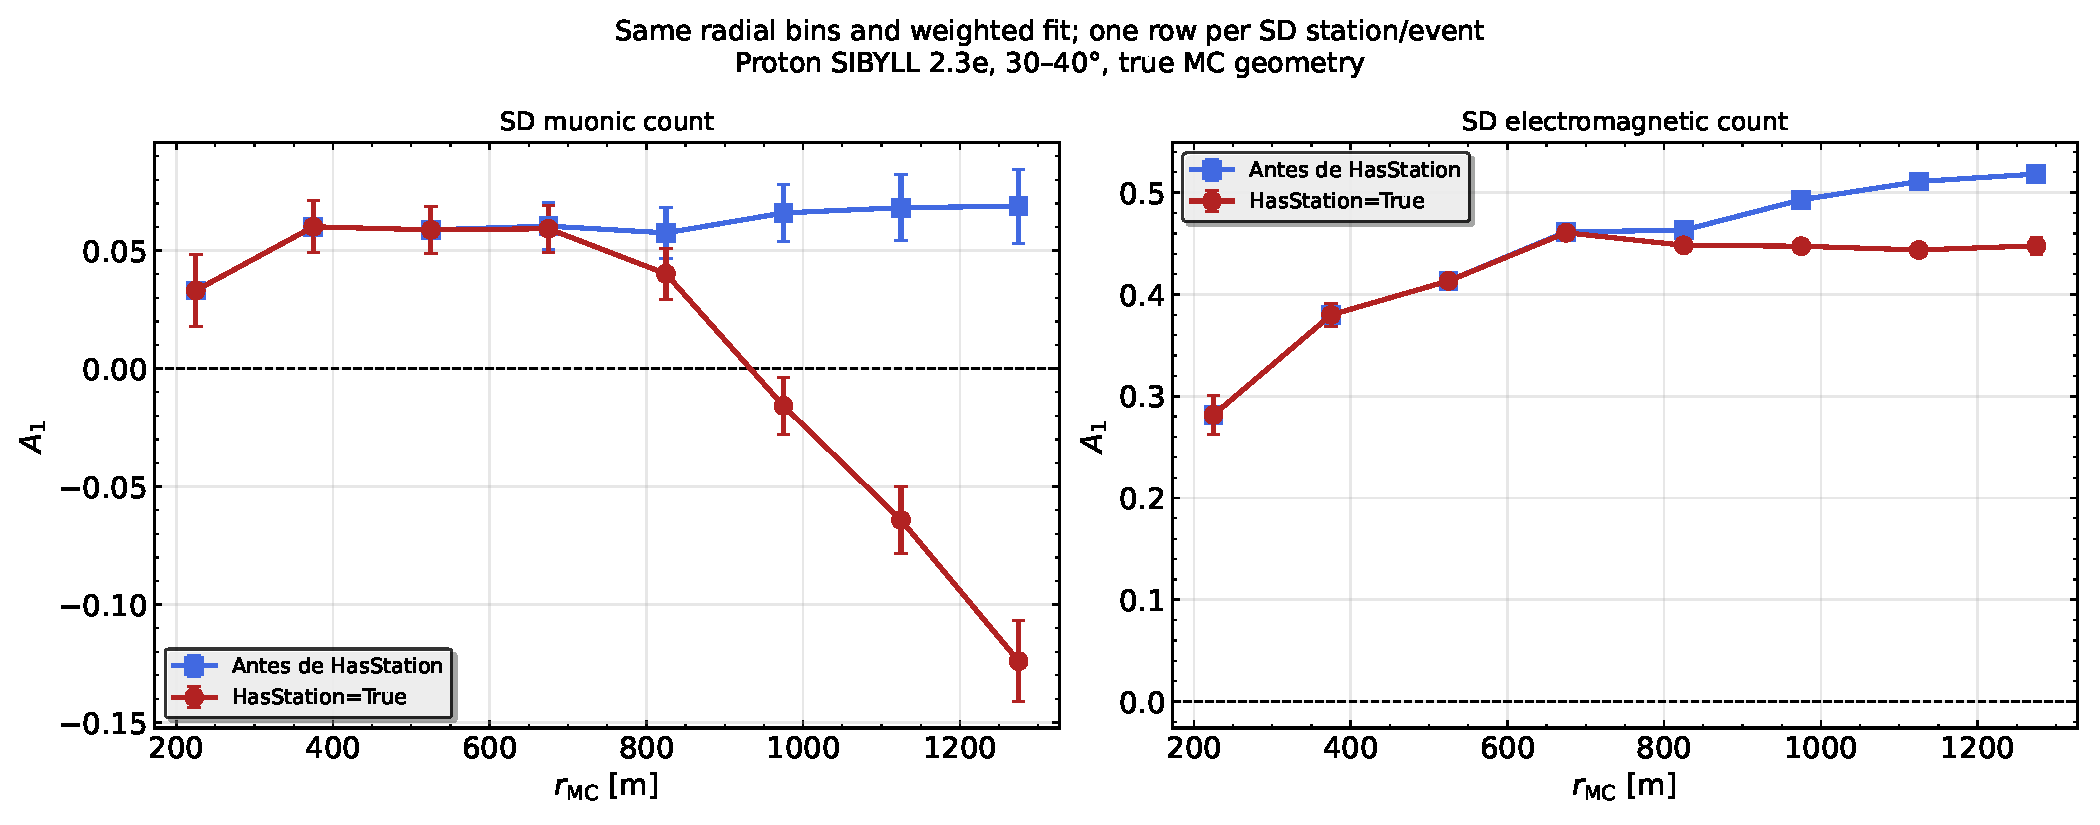
\includegraphics[width=\textwidth]{claude_work/revision_asimetrias_sd_umd/02_notebooks/02_reproduccion/resultados/SD_antes_despues_mismos_bins.pdf}
\caption{Control de la selección SD con geometría Monte Carlo y el mismo bineado radial y azimutal a ambos lados del corte. El conteo muónico permanece positivo antes de exigir \texttt{HasStation} e invierte su signo después. La componente electromagnética permanece positiva, aunque su amplitud también cambia. Las barras de esta figura reproducen los errores formales del ajuste ponderado original; la Tabla~\ref{tab:infill2026_comparacion} utiliza incertidumbres por remuestreo de lluvias.}
\label{fig:infill2026_antes_despues}
\end{figure}

El resultado del intervalo exterior se resume en la Tabla~\ref{tab:infill2026_comparacion}. Se conserva el conteo UMD de la selección original como referencia, sin presentarlo como una muestra subterránea no seleccionada.

Las incertidumbres de esta comparación se obtienen mediante $1200$ réplicas
pareadas sobre $960$ grupos de lluvia progenitora identificados en la muestra.
En cada réplica se mantienen juntas sus reutilizaciones y se recalculan las
medias azimutales, sus errores y el ajuste para los tres observables. Este
agrupamiento utiliza los identificadores disponibles y no sustituye una
auditoría completa de la genealogía de las simulaciones.

\begin{table}[H]
\centering
\begin{tabular}{lcc}
\toprule
Observable y selección & $A_1$ & $\sigma_{\mathrm{bootstrap}}$\\
\midrule
SD muónico antes de \texttt{HasStation} & $+0.0689$ & $0.0157$\\
SD muónico con \texttt{HasStation} & $-0.1240$ & $0.0186$\\
UMD, selección original & $+0.0816$ & $0.0344$\\
\bottomrule
\end{tabular}
\caption{Comparación para $1200\leq r<1350$~m y $30^\circ\leq\theta<40^\circ$. Las incertidumbres son desviaciones estándar de un \textit{bootstrap} que conserva conjuntamente las estaciones, módulos y reutilizaciones agrupadas por identificador de lluvia progenitora. No son las incertidumbres formales del ajuste a medias independientes. Los coeficientes no deben confundirse con valores ilustrativos citados anteriormente a radio nominal $r\simeq1200$~m y con otro bineado.}
\label{tab:infill2026_comparacion}
\end{table}

En esta corona el conjunto SD pasa de $12212$ a $3694$ registros al aplicar la condición. El cambio de signo se obtiene sin modificar sus conteos, sus coordenadas Monte Carlo ni el estimador. Por lo tanto, la selección es suficiente para producir la inversión observada en esta muestra. No es necesario introducir un nuevo término atmosférico negativo para explicar la diferencia entre esos dos promedios.

La comparación con UMD tampoco debe reducirse a que ambos coeficientes anteriores al corte sean positivos. En el intervalo de la tabla, la diferencia pareada SD antes del corte menos UMD es $-0.0127$, con intervalo percentil puntual del $95\%$ de $[-0.0897,+0.0555]$. No se resuelve allí una diferencia con ese procedimiento, pero ello no prueba igualdad física. En coronas interiores sí aparecen diferencias, por lo que retirar \texttt{HasStation} no vuelve idénticas las curvas de ambos instrumentos. El remuestreo contempla la dependencia entre registros de una lluvia, no las incertidumbres sistemáticas del detector o del modelo hadrónico.

\subsubsection{Interpretación física: selección dependiente de la señal}

Una hipótesis coherente con el signo observado es el acoplamiento entre la componente electromagnética y la condición que retiene una estación. En la región temprana, una contribución electromagnética mayor puede ayudar a retener estaciones aun con pocos muones. En la tardía, con menor contribución electromagnética, las estaciones que sobreviven pueden estar enriquecidas en fluctuaciones muónicas positivas. El promedio de muones por estación retenida puede resultar entonces mayor en la región tardía, aunque el promedio previo favorezca la temprana.

La atenuación electromagnética participaría así de forma indirecta, modificando la señal que favorece la selección; no cambia el signo de las pérdidas pasivas de muones. Tampoco se confunden electrones con muones: cambia el conjunto de estaciones en el que se promedian los muones verdaderos.

El cambio de signo al aplicar \texttt{HasStation} es un resultado del control. La secuencia particular de ayuda electromagnética y enriquecimiento muónico es una interpretación física pendiente de aislamiento causal. \texttt{HasStation} informa presencia en la colección reconstruida y no identifica, por sí solo, un único umbral de disparo ni una etapa específica de reconstrucción. El resultado no demuestra un error del programa \textit{Offline}: una selección correctamente implementada puede sesgar una media si se la interpreta como incondicional.

\subsection{Qué establece la comparación con el UMD}
\label{subsec:umd_poblacion_seleccion}

El UMD y el SD no muestrean la misma apertura ni la misma población de cruces. El suelo modifica las distribuciones de energía y dirección de los muones que alcanzan los centelladores. Por otra parte, los muones contabilizados por el SD contribuyen directamente a la señal del tanque que interviene en la selección. Un muón que atraviesa un módulo enterrado cercano no es, en general, el mismo que atraviesa el tanque. La correlación de cada conteo con la selección SD puede, por ello, ser diferente, aun cuando ambos estén correlacionados por pertenecer a la misma lluvia.

Estas diferencias permiten comprender por qué no es obligatorio que el UMD reproduzca la inversión del SD seleccionado. No prueban que el UMD esté libre de selección ni que su exceso temprano sea exclusivamente atmosférico. La concordancia aproximada de un modelo de transporte y apertura con una amplitud UMD tampoco reemplaza el control de la población efectivamente observada.

Con los resúmenes disponibles no se ha construido una comparación UMD equivalente a la de la Figura~\ref{fig:infill2026_antes_despues}. La auditoría de los objetos ADST identificó que la verdad de los centelladores puede no quedar serializada cuando no se crean los canales electrónicos asociados al disparo SD. Un contador ausente o una suma sobre una lista vacía no demuestran que no hayan atravesado muones el módulo. Los ceros conservados por compatibilidad con el lector original no deben convertirse en ceros físicos de una población UMD no seleccionada. Recuperar más filas sin \texttt{HasStation} tampoco resuelve por sí solo esa falta de información.

\subsection{Geometría reconstruida: un sistemático distinto}
\label{subsec:infill_rec}

Se reemplazan ahora el núcleo y la dirección verdaderos por sus valores reconstruidos. Aun manteniendo las mismas estaciones, cambian el radio y el azimut asignados a cada una y pueden producirse migraciones entre coronas. Este efecto es distinto del anterior: la selección modifica qué estaciones entran, mientras que la reconstrucción geométrica modifica dónde se ubican las que entran.

En las comparaciones originales, el cambio de conteo MC a REC con geometría fija conserva gran parte de la tendencia del UMD. Al cambiar también las coordenadas, la extracción se degrada en varias regiones, especialmente cuando la amplitud es pequeña o el gradiente radial es grande. Las grillas con geometría reconstruida documentan ese comportamiento; no se asume que la pérdida sea uniforme ni que exista una ventana óptima universal.

Un modelo de errores de fase independientes del conteo y del azimut verdadero, simétricos y sin migración radial daría $A_1^{\mathrm{REC}}=A_1^{\mathrm{MC}}\langle\cos\Delta\phi\rangle$. Este límite ilustra una atenuación por mezcla angular, pero los errores reales del núcleo también tienen estructura direccional. En el control con estaciones del Infill mostrado en la presentación RAFA y en la Figura~\ref{fig:bias_core_azimut}, $\Delta r=r_{\mathrm{MC}}-r_{\mathrm{REC}}$ es negativo en la región temprana y positivo en la tardía. A dirección fija, el patrón es compatible con un desplazamiento del núcleo reconstruido hacia el lado tardío; las diferencias de dirección y las migraciones de muestra deben controlarse para cuantificarlo.

Una LDF que no representa explícitamente la modulación azimutal puede absorber parte de ella mediante ajustes de posición y de otros parámetros. Esta interpretación debe distinguirse del modelo de remuestreo de residuos de conteo de la Sección~\ref{subsec:toy_model}: ese modelo cuantifica cómo una respuesta direccional del conteo modifica $A_1$, pero no vuelve a ejecutar la reconstrucción del núcleo y no demuestra por sí solo toda la cadena causal propuesta para su desplazamiento.

La componente electromagnética puede seguir mostrando una modulación positiva significativa bajo geometría reconstruida. Una amplitud mayor y errores estadísticos menores facilitan su detección, pero la abundancia de partículas no elimina un sesgo de coordenadas. Asimismo, la persistencia de un coeficiente SD negativo no exige una población de muones blandos con proyección negativa: la muestra sigue condicionada por selección, y la geometría reconstruida puede modificar ese coeficiente sin eliminar su signo.

\subsection{Alcance de los resultados y controles restantes}
\label{subsec:comparacion_performance_umd}
\label{subsec:fast_mc}

Una evaluación MC--REC completa debe comparar, sobre una muestra emparejada, el cambio de conteo a geometría fija y el cambio de geometría a conteo fijo. Las diferencias de amplitud deben incluir sus covarianzas y las migraciones radiales; un cociente resulta inestable cuando el coeficiente de referencia es cercano a cero. En presencia de sesgos correlacionados, ni $A_1^{\mathrm{REC}}$ es una cota inferior universal ni $A_1^{\mathrm{MC}}$ una cota superior universal.

El resultado central de este capítulo es que la condición de presencia de estación reconstruida induce la inversión del promedio muónico SD en la muestra auditada. La física de propagación, la proyección y la respuesta del tanque siguen siendo necesarias para predecir las poblaciones y sus señales; la selección debe aplicarse además para predecir el observable realmente ajustado. No se establece una inversión universal del flujo al suelo ni un fallo de reconstrucción instrumental.

Los controles siguientes tienen requisitos de información diferentes. Extender la prueba SD a otros primarios, energías e inclinaciones requiere repetir la comparación sobre sus estaciones simuladas. Separar las etapas responsables de la selección requiere sus estados de disparo, lectura y reconstrucción junto con conteos y señales. Para obtener el control UMD se necesita conservar el conteo anterior a la electrónica, distinguiendo explícitamente cero de dato ausente. Ninguna de estas preguntas exige cinemática individual de producción.

En cambio, una predicción desde producción necesita la distribución conjunta de profundidad, energía y momento transversal, con sus correlaciones y su transporte hasta los detectores \cite{Cazon2012}. Esa información no puede reconstruirse únicamente a partir de los conteos agregados de los ADST. El propagador fenomenológico previo no resolvió esa limitación y no constituye una validación de la antigua explicación de muones blandos. La sensibilidad a composición y energía del Infill, así como la transferencia a datos reales, quedan sujetas a controles propios; no se deducen automáticamente del resultado favorable del Anillo Denso ni de la prueba de selección presentada aquí.

\newpage
